\documentclass[tikz,border=8pt]{standalone}
\usepackage[utf8]{inputenc}
\usepackage{amsmath}
\usetikzlibrary{arrows.meta, positioning, calc}
\renewcommand{\familydefault}{\sfdefault}
\begin{document}
	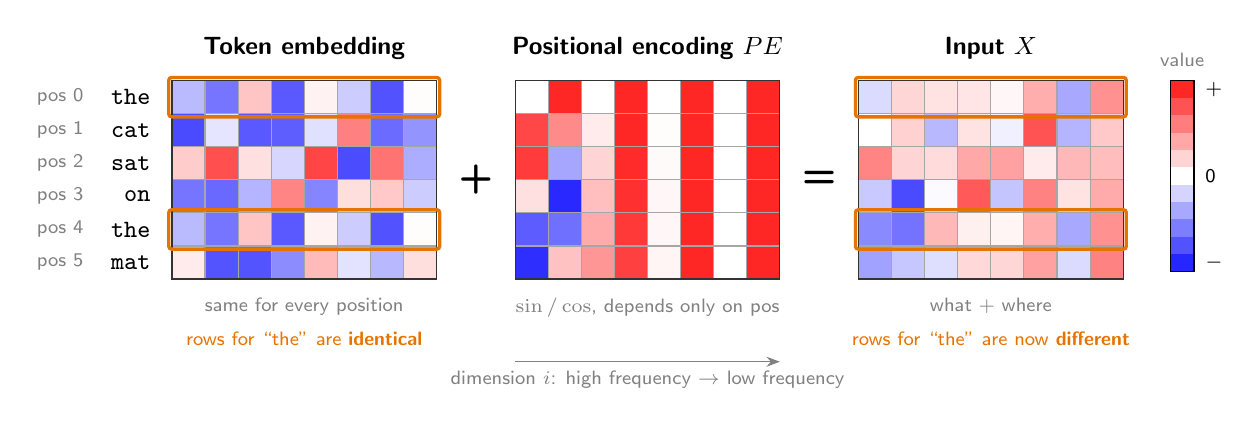
\begin{tikzpicture}[
		ttl/.style={font=\sffamily\small\bfseries, anchor=south},
		sub/.style={font=\sffamily\scriptsize, text=gray, anchor=north},
		op/.style={font=\sffamily\Large\bfseries}
		]
		\node[anchor=east, font=\ttfamily\small] at (-0.15,-0.210) {the};
		\node[anchor=east, font=\sffamily\scriptsize, text=gray] at (-1.0,-0.210) {pos 0};
		\node[anchor=east, font=\ttfamily\small] at (-0.15,-0.630) {cat};
		\node[anchor=east, font=\sffamily\scriptsize, text=gray] at (-1.0,-0.630) {pos 1};
		\node[anchor=east, font=\ttfamily\small] at (-0.15,-1.050) {sat};
		\node[anchor=east, font=\sffamily\scriptsize, text=gray] at (-1.0,-1.050) {pos 2};
		\node[anchor=east, font=\ttfamily\small] at (-0.15,-1.470) {on};
		\node[anchor=east, font=\sffamily\scriptsize, text=gray] at (-1.0,-1.470) {pos 3};
		\node[anchor=east, font=\ttfamily\small] at (-0.15,-1.890) {the};
		\node[anchor=east, font=\sffamily\scriptsize, text=gray] at (-1.0,-1.890) {pos 4};
		\node[anchor=east, font=\ttfamily\small] at (-0.15,-2.310) {mat};
		\node[anchor=east, font=\sffamily\scriptsize, text=gray] at (-1.0,-2.310) {pos 5};
		\fill[blue!27!white] (0.000,0.000) rectangle ++(0.42,-0.42);
		\fill[blue!54!white] (0.420,0.000) rectangle ++(0.42,-0.42);
		\fill[red!23!white] (0.840,0.000) rectangle ++(0.42,-0.42);
		\fill[blue!65!white] (1.260,0.000) rectangle ++(0.42,-0.42);
		\fill[red!5!white] (1.680,0.000) rectangle ++(0.42,-0.42);
		\fill[blue!20!white] (2.100,0.000) rectangle ++(0.42,-0.42);
		\fill[blue!68!white] (2.520,0.000) rectangle ++(0.42,-0.42);
		\fill[red!1!white] (2.940,0.000) rectangle ++(0.42,-0.42);
		\fill[blue!71!white] (0.000,-0.420) rectangle ++(0.42,-0.42);
		\fill[blue!10!white] (0.420,-0.420) rectangle ++(0.42,-0.42);
		\fill[blue!65!white] (0.840,-0.420) rectangle ++(0.42,-0.42);
		\fill[blue!63!white] (1.260,-0.420) rectangle ++(0.42,-0.42);
		\fill[blue!12!white] (1.680,-0.420) rectangle ++(0.42,-0.42);
		\fill[red!50!white] (2.100,-0.420) rectangle ++(0.42,-0.42);
		\fill[blue!58!white] (2.520,-0.420) rectangle ++(0.42,-0.42);
		\fill[blue!42!white] (2.940,-0.420) rectangle ++(0.42,-0.42);
		\fill[red!20!white] (0.000,-0.840) rectangle ++(0.42,-0.42);
		\fill[red!69!white] (0.420,-0.840) rectangle ++(0.42,-0.42);
		\fill[red!12!white] (0.840,-0.840) rectangle ++(0.42,-0.42);
		\fill[blue!16!white] (1.260,-0.840) rectangle ++(0.42,-0.42);
		\fill[red!73!white] (1.680,-0.840) rectangle ++(0.42,-0.42);
		\fill[blue!70!white] (2.100,-0.840) rectangle ++(0.42,-0.42);
		\fill[red!55!white] (2.520,-0.840) rectangle ++(0.42,-0.42);
		\fill[blue!32!white] (2.940,-0.840) rectangle ++(0.42,-0.42);
		\fill[blue!54!white] (0.000,-1.260) rectangle ++(0.42,-0.42);
		\fill[blue!59!white] (0.420,-1.260) rectangle ++(0.42,-0.42);
		\fill[blue!29!white] (0.840,-1.260) rectangle ++(0.42,-0.42);
		\fill[red!48!white] (1.260,-1.260) rectangle ++(0.42,-0.42);
		\fill[blue!48!white] (1.680,-1.260) rectangle ++(0.42,-0.42);
		\fill[red!13!white] (2.100,-1.260) rectangle ++(0.42,-0.42);
		\fill[red!21!white] (2.520,-1.260) rectangle ++(0.42,-0.42);
		\fill[blue!20!white] (2.940,-1.260) rectangle ++(0.42,-0.42);
		\fill[blue!27!white] (0.000,-1.680) rectangle ++(0.42,-0.42);
		\fill[blue!54!white] (0.420,-1.680) rectangle ++(0.42,-0.42);
		\fill[red!23!white] (0.840,-1.680) rectangle ++(0.42,-0.42);
		\fill[blue!65!white] (1.260,-1.680) rectangle ++(0.42,-0.42);
		\fill[red!5!white] (1.680,-1.680) rectangle ++(0.42,-0.42);
		\fill[blue!20!white] (2.100,-1.680) rectangle ++(0.42,-0.42);
		\fill[blue!68!white] (2.520,-1.680) rectangle ++(0.42,-0.42);
		\fill[red!1!white] (2.940,-1.680) rectangle ++(0.42,-0.42);
		\fill[red!8!white] (0.000,-2.100) rectangle ++(0.42,-0.42);
		\fill[blue!67!white] (0.420,-2.100) rectangle ++(0.42,-0.42);
		\fill[blue!67!white] (0.840,-2.100) rectangle ++(0.42,-0.42);
		\fill[blue!45!white] (1.260,-2.100) rectangle ++(0.42,-0.42);
		\fill[red!27!white] (1.680,-2.100) rectangle ++(0.42,-0.42);
		\fill[blue!11!white] (2.100,-2.100) rectangle ++(0.42,-0.42);
		\fill[blue!28!white] (2.520,-2.100) rectangle ++(0.42,-0.42);
		\fill[red!13!white] (2.940,-2.100) rectangle ++(0.42,-0.42);
		\draw[step=0.42, black!35, shift={(0,0)}] (0,0) grid (3.360,-2.520);
		\draw[black!80] (0,0) rectangle ++(3.360,-2.520);
		\coordinate (E) at (1.680,0);
		\node[ttl] at (1.680,0.15) {Token embedding};
		\node[sub] at (1.680,-2.640) {same for every position};
		\node[op] at (3.860,-1.260) {+};
		\fill[red!0!white] (4.360,0.000) rectangle ++(0.42,-0.42);
		\fill[red!85!white] (4.780,0.000) rectangle ++(0.42,-0.42);
		\fill[red!0!white] (5.200,0.000) rectangle ++(0.42,-0.42);
		\fill[red!85!white] (5.620,0.000) rectangle ++(0.42,-0.42);
		\fill[red!0!white] (6.040,0.000) rectangle ++(0.42,-0.42);
		\fill[red!85!white] (6.460,0.000) rectangle ++(0.42,-0.42);
		\fill[red!0!white] (6.880,0.000) rectangle ++(0.42,-0.42);
		\fill[red!85!white] (7.300,0.000) rectangle ++(0.42,-0.42);
		\fill[red!72!white] (4.360,-0.420) rectangle ++(0.42,-0.42);
		\fill[red!46!white] (4.780,-0.420) rectangle ++(0.42,-0.42);
		\fill[red!8!white] (5.200,-0.420) rectangle ++(0.42,-0.42);
		\fill[red!85!white] (5.620,-0.420) rectangle ++(0.42,-0.42);
		\fill[red!1!white] (6.040,-0.420) rectangle ++(0.42,-0.42);
		\fill[red!85!white] (6.460,-0.420) rectangle ++(0.42,-0.42);
		\fill[red!0!white] (6.880,-0.420) rectangle ++(0.42,-0.42);
		\fill[red!85!white] (7.300,-0.420) rectangle ++(0.42,-0.42);
		\fill[red!77!white] (4.360,-0.840) rectangle ++(0.42,-0.42);
		\fill[blue!35!white] (4.780,-0.840) rectangle ++(0.42,-0.42);
		\fill[red!17!white] (5.200,-0.840) rectangle ++(0.42,-0.42);
		\fill[red!83!white] (5.620,-0.840) rectangle ++(0.42,-0.42);
		\fill[red!2!white] (6.040,-0.840) rectangle ++(0.42,-0.42);
		\fill[red!85!white] (6.460,-0.840) rectangle ++(0.42,-0.42);
		\fill[red!0!white] (6.880,-0.840) rectangle ++(0.42,-0.42);
		\fill[red!85!white] (7.300,-0.840) rectangle ++(0.42,-0.42);
		\fill[red!12!white] (4.360,-1.260) rectangle ++(0.42,-0.42);
		\fill[blue!84!white] (4.780,-1.260) rectangle ++(0.42,-0.42);
		\fill[red!25!white] (5.200,-1.260) rectangle ++(0.42,-0.42);
		\fill[red!81!white] (5.620,-1.260) rectangle ++(0.42,-0.42);
		\fill[red!3!white] (6.040,-1.260) rectangle ++(0.42,-0.42);
		\fill[red!85!white] (6.460,-1.260) rectangle ++(0.42,-0.42);
		\fill[red!0!white] (6.880,-1.260) rectangle ++(0.42,-0.42);
		\fill[red!85!white] (7.300,-1.260) rectangle ++(0.42,-0.42);
		\fill[blue!64!white] (4.360,-1.680) rectangle ++(0.42,-0.42);
		\fill[blue!56!white] (4.780,-1.680) rectangle ++(0.42,-0.42);
		\fill[red!33!white] (5.200,-1.680) rectangle ++(0.42,-0.42);
		\fill[red!78!white] (5.620,-1.680) rectangle ++(0.42,-0.42);
		\fill[red!3!white] (6.040,-1.680) rectangle ++(0.42,-0.42);
		\fill[red!85!white] (6.460,-1.680) rectangle ++(0.42,-0.42);
		\fill[red!0!white] (6.880,-1.680) rectangle ++(0.42,-0.42);
		\fill[red!85!white] (7.300,-1.680) rectangle ++(0.42,-0.42);
		\fill[blue!82!white] (4.360,-2.100) rectangle ++(0.42,-0.42);
		\fill[red!24!white] (4.780,-2.100) rectangle ++(0.42,-0.42);
		\fill[red!41!white] (5.200,-2.100) rectangle ++(0.42,-0.42);
		\fill[red!75!white] (5.620,-2.100) rectangle ++(0.42,-0.42);
		\fill[red!4!white] (6.040,-2.100) rectangle ++(0.42,-0.42);
		\fill[red!85!white] (6.460,-2.100) rectangle ++(0.42,-0.42);
		\fill[red!0!white] (6.880,-2.100) rectangle ++(0.42,-0.42);
		\fill[red!85!white] (7.300,-2.100) rectangle ++(0.42,-0.42);
		\draw[step=0.42, black!35, shift={(4.359999999999999,0)}] (0,0) grid (3.360,-2.520);
		\draw[black!80] (4.359999999999999,0) rectangle ++(3.360,-2.520);
		\coordinate (P) at (6.040,0);
		\node[ttl] at (6.040,0.15) {Positional encoding $PE$};
		\node[sub] at (6.040,-2.640) {$\sin/\cos$, depends only on pos};
		\node[op] at (8.220,-1.260) {=};
		\fill[blue!14!white] (8.720,0.000) rectangle ++(0.42,-0.42);
		\fill[red!16!white] (9.140,0.000) rectangle ++(0.42,-0.42);
		\fill[red!11!white] (9.560,0.000) rectangle ++(0.42,-0.42);
		\fill[red!10!white] (9.980,0.000) rectangle ++(0.42,-0.42);
		\fill[red!3!white] (10.400,0.000) rectangle ++(0.42,-0.42);
		\fill[red!32!white] (10.820,0.000) rectangle ++(0.42,-0.42);
		\fill[blue!34!white] (11.240,0.000) rectangle ++(0.42,-0.42);
		\fill[red!43!white] (11.660,0.000) rectangle ++(0.42,-0.42);
		\fill[red!0!white] (8.720,-0.420) rectangle ++(0.42,-0.42);
		\fill[red!18!white] (9.140,-0.420) rectangle ++(0.42,-0.42);
		\fill[blue!28!white] (9.560,-0.420) rectangle ++(0.42,-0.42);
		\fill[red!11!white] (9.980,-0.420) rectangle ++(0.42,-0.42);
		\fill[blue!6!white] (10.400,-0.420) rectangle ++(0.42,-0.42);
		\fill[red!68!white] (10.820,-0.420) rectangle ++(0.42,-0.42);
		\fill[blue!29!white] (11.240,-0.420) rectangle ++(0.42,-0.42);
		\fill[red!21!white] (11.660,-0.420) rectangle ++(0.42,-0.42);
		\fill[red!48!white] (8.720,-0.840) rectangle ++(0.42,-0.42);
		\fill[red!17!white] (9.140,-0.840) rectangle ++(0.42,-0.42);
		\fill[red!14!white] (9.560,-0.840) rectangle ++(0.42,-0.42);
		\fill[red!34!white] (9.980,-0.840) rectangle ++(0.42,-0.42);
		\fill[red!37!white] (10.400,-0.840) rectangle ++(0.42,-0.42);
		\fill[red!8!white] (10.820,-0.840) rectangle ++(0.42,-0.42);
		\fill[red!28!white] (11.240,-0.840) rectangle ++(0.42,-0.42);
		\fill[red!26!white] (11.660,-0.840) rectangle ++(0.42,-0.42);
		\fill[blue!21!white] (8.720,-1.260) rectangle ++(0.42,-0.42);
		\fill[blue!71!white] (9.140,-1.260) rectangle ++(0.42,-0.42);
		\fill[blue!2!white] (9.560,-1.260) rectangle ++(0.42,-0.42);
		\fill[red!65!white] (9.980,-1.260) rectangle ++(0.42,-0.42);
		\fill[blue!23!white] (10.400,-1.260) rectangle ++(0.42,-0.42);
		\fill[red!49!white] (10.820,-1.260) rectangle ++(0.42,-0.42);
		\fill[red!11!white] (11.240,-1.260) rectangle ++(0.42,-0.42);
		\fill[red!33!white] (11.660,-1.260) rectangle ++(0.42,-0.42);
		\fill[blue!46!white] (8.720,-1.680) rectangle ++(0.42,-0.42);
		\fill[blue!55!white] (9.140,-1.680) rectangle ++(0.42,-0.42);
		\fill[red!28!white] (9.560,-1.680) rectangle ++(0.42,-0.42);
		\fill[red!6!white] (9.980,-1.680) rectangle ++(0.42,-0.42);
		\fill[red!4!white] (10.400,-1.680) rectangle ++(0.42,-0.42);
		\fill[red!32!white] (10.820,-1.680) rectangle ++(0.42,-0.42);
		\fill[blue!34!white] (11.240,-1.680) rectangle ++(0.42,-0.42);
		\fill[red!43!white] (11.660,-1.680) rectangle ++(0.42,-0.42);
		\fill[blue!37!white] (8.720,-2.100) rectangle ++(0.42,-0.42);
		\fill[blue!22!white] (9.140,-2.100) rectangle ++(0.42,-0.42);
		\fill[blue!13!white] (9.560,-2.100) rectangle ++(0.42,-0.42);
		\fill[red!15!white] (9.980,-2.100) rectangle ++(0.42,-0.42);
		\fill[red!16!white] (10.400,-2.100) rectangle ++(0.42,-0.42);
		\fill[red!37!white] (10.820,-2.100) rectangle ++(0.42,-0.42);
		\fill[blue!14!white] (11.240,-2.100) rectangle ++(0.42,-0.42);
		\fill[red!49!white] (11.660,-2.100) rectangle ++(0.42,-0.42);
		\draw[step=0.42, black!35, shift={(8.719999999999999,0)}] (0,0) grid (3.360,-2.520);
		\draw[black!80] (8.719999999999999,0) rectangle ++(3.360,-2.520);
		\coordinate (X) at (10.400,0);
		\node[ttl] at (10.400,0.15) {Input $X$};
		\node[sub] at (10.400,-2.640) {what + where};
		\draw[orange!90!black, very thick, rounded corners=1pt] (-0.040,0.040) rectangle ++(3.440,-0.500);
		\draw[orange!90!black, very thick, rounded corners=1pt] (-0.040,-1.640) rectangle ++(3.440,-0.500);
		\draw[orange!90!black, very thick, rounded corners=1pt] (8.680,0.040) rectangle ++(3.440,-0.500);
		\draw[orange!90!black, very thick, rounded corners=1pt] (8.680,-1.640) rectangle ++(3.440,-0.500);
		\node[font=\sffamily\scriptsize, text=orange!90!black, anchor=north, align=center] at (1.680,-3.070) {rows for ``the'' are \textbf{identical}};
		\node[font=\sffamily\scriptsize, text=orange!90!black, anchor=north, align=center] at (10.400,-3.070) {rows for ``the'' are now \textbf{different}};
		\draw[-{Stealth}, gray] (4.360,-3.570) -- (7.720,-3.570) node[midway, below, font=\sffamily\scriptsize, text=gray] {dimension $i$: high frequency $\rightarrow$ low frequency};
		\fill[red!85!white] (12.680,0.000) rectangle ++(0.3,-0.22);
		\fill[red!68!white] (12.680,-0.220) rectangle ++(0.3,-0.22);
		\fill[red!51!white] (12.680,-0.440) rectangle ++(0.3,-0.22);
		\fill[red!34!white] (12.680,-0.660) rectangle ++(0.3,-0.22);
		\fill[red!17!white] (12.680,-0.880) rectangle ++(0.3,-0.22);
		\fill[red!0!white] (12.680,-1.100) rectangle ++(0.3,-0.22);
		\fill[blue!17!white] (12.680,-1.320) rectangle ++(0.3,-0.22);
		\fill[blue!34!white] (12.680,-1.540) rectangle ++(0.3,-0.22);
		\fill[blue!51!white] (12.680,-1.760) rectangle ++(0.3,-0.22);
		\fill[blue!68!white] (12.680,-1.980) rectangle ++(0.3,-0.22);
		\fill[blue!85!white] (12.680,-2.200) rectangle ++(0.3,-0.22);
		\draw (12.680,0) rectangle ++(0.3,-2.420);
		\node[anchor=west,font=\sffamily\scriptsize] at (13.000,-0.11) {$+$};
		\node[anchor=west,font=\sffamily\scriptsize] at (13.000,-2.310) {$-$};
		\node[anchor=west,font=\sffamily\scriptsize] at (13.000,-1.210) {0};
		\node[anchor=south,font=\sffamily\scriptsize,text=gray] at (12.830,0.05) {value};
	\end{tikzpicture}
\end{document}